\section{Experiments}
\subsection{Experimental Setup}
%\textbf{Dataset and Evaluation Methodology}. 
We use Freebase and the English Wikipedia dump of 2016-11-20, to construct our dataset. Statistics for the generated dataset is shown in Table~\ref{statistics}. Note that all sentences in the dataset are positive. 
\begin{table}
\small
\centering
\begin{tabular}{|l|c|c|c|} \hline
& Train & Dev & Test \\ \hline
\emph{\#Sent.} & 4800 & 1200 & 1180 \\ \hline
\emph{\#Eve.} & 4918 & 1247 & 1229 \\ \hline
\emph{\#Arg.} & 17274 & 4318 & 4248 \\ \hline
\emph{\%Multi\_Eve.} & 3.0 & 3.2 & 3.1 \\ \hline
% \emph{\%Multi\_Arg.} & 67.4 & 67.0 & 67.9 \\ \hline
\end{tabular}	
\caption{Statistics for the generated dataset. \emph{\#Sent.} is the number of sentences, \emph{\#Eve.} is the number of event mentions, and \emph{\#Arg.} is the number of event arguments. \emph{\%Multi\_Eve.} is the ratio of multi-type events.
%, and \emph{\%Multi\_Arg.} is the ratio of multi-word arguments.
\label{statistics}}
\end{table}
% containing 7,180 sentences, containing 7,394 events and 25,840 arguments. We then randomly select 4,800 sentences for training and 1,180 sentences as test set, and the rest 1,200 sentences for validation. 
We first manually evaluate the quality of our test set and then regard the automatically generated data as gold standard and evaluate our model accordingly. Next, we manually evaluate a subset of events detected by our model and analyze the differences with regards to the automatic evaluation. Finally, we conduct evaluation on a smaller dataset annotated by tables crawled from Wikipedia's pages. 

\paragraph{Evaluation Measures} We evaluate our models in terms of precision (P), recall (R), and F-measure (F) for each subtask. These performance metrics are computed according to the following standards of correctness: 
For \emph{event type classification}, an event is correctly classified if its reference sentence contains all key arguments of this event type. 
For \emph{argument detection}, an argument is correctly detected if its offsets, role, and related event type exactly match the reference argument within the same sentence. 
For \emph{event detection}, an event is correctly detected if its type and all its key arguments match a reference event within the same sentence.

\paragraph{Training} All hyper-parameters are tuned on the development set. In event detection, we set the size of word embeddings to 200, the size of LSTM layer to 100. In argument detection, we use the same size of word embedding, while the size of LSTM layer is 150, and the size of key argument embedding is 50. Word embeddings are pre-trained using skip-gram word2vec~\cite{mikolov2013distributed} on English Wikipedia pages and fine tuned during training. To mitigate overfitting, we apply a dropout rate of 0.5 on both the input and output layers.

\subsection{Dataset Evaluation}\label{sec:evalhypo}
To investigate the possibility of automatically constructing training data for event extraction, we evaluate five datasets that utilize  following strategies to determine key arguments and collect positive sentences from Wikipedia pages: (1) \emph{ALL} means regarding all arguments as key arguments; (2) \emph{IMP} means selecting the top half arguments with high importance value as key arguments; (3) \emph{IMP\&TIME} means adding a time-related argument with highest importance value to the set of key arguments generated by \emph{IMP}; (4) \emph{DIS} means eliminating sentence where dependency distances between any two key arguments are greater than 2. We randomly select 100 sentences in each dataset, and annotators are asked to determine whether each sentence implies a given event.

% 怎么介绍Strategy比较省地方?
\begin{table}[h]
\small
\centering
\begin{tabular}{|c|l|c|c|c|} \hline
	No. & Selection strategy & Dataset & Type & Pos \\ \hline
	S1 & \emph{ALL} & 203 & 9 & 98 \\ \hline
	S2 & \emph{IMP} & 108K & 24 & 22 \\ \hline
	S3 & \emph{IMP} + \emph{DIS} & 12K & 24 & 37 \\ \hline
	S4 & \emph{IMP\&TIME} & 9241 & 24 & 81 \\ \hline
	S5 & \emph{IMP\&TIME} + \emph{DIS} & 7180 & 24 & 89 \\ \hline
	% Instances & 0.3M & 3.6M & 3.6M & 1.3M & 1.3M \\ \hline
	% Dataset & 203 & 108K & 12K & 9241 & 7180 \\ \hline
	% Event type & 9 & 24 & 24 & 24 & 24 \\ \hline
	% Correct (\%) & 98 & 22 & 37 & 81 & 89 \\ \hline
\end{tabular}
\caption{Statistic of the datasets built with different strategies. 
% \textit{Instances} denotes the number of CVT instances that can be used for each hypothesis. 
\textit{Dataset} is the number of sentences found. \textit{Type} indicates the number of different CVT types in each dataset.  \textit{Pos} is the percentage of sentences mentioning the given events explicitly. \label{tab:3}}
\end{table}

As shown in Table~\ref{tab:3}, it is not surprising that the most strict strategy, \emph{S1}, guarantees the quality of the generated data, while we can merely obtain 203 sentences covering 9 types of events, which is insufficient for further applications. \emph{S2} relaxes \emph{S1} by allowing the absence of non-key arguments, which expands the resulting dataset, but introduces more noise into the dataset. 
This side effect indicates that \emph{S2} is inappropriate to be used as a soft constraint. Compared with \emph{S2}, the significant improvement in the quality of sentences collected by \emph{S4} proves that time-related arguments within CVT schemas are critical to imply an event occurrence. Among all strategies, data obtained by \emph{S5} achieves the highest precision, while still accounting for 7,180 sentences, showing that it is feasible to automatically collect quality training data for event extraction without either human-designed event schemas or extra human annotations.     
% our hypothesis \emph{H3} and \emph{H4} are feasible and it is an effective way to generate reliable data automatically.

\subsection{Baselines}
%To investigate the effectiveness of our proposed model, 
We compare our proposed models with three baseline extraction systems, including traditional feature-based methods and neural network models. All baselines are trained following the two-step pipeline, i.e., event detection and argument detection.
For neural network method, we train a simple LSTM model that takes word embeddings as input, and outputs the label with the maximum probability among all possible labels. 
For feature-based methods, we apply Conditional Random Field \cite{lafferty2001conditional} and Maximum Entropy \cite{berger1996maximum} to explore a variety of elaborate features, such as lexical, syntactic and entity-related features, according to the state-of-art feature-based ACE event extraction system~\cite{li2013joint}. Note that during argument detection stage, we add the label of each word output by event detection as a supplementary feature.
We use Stanford CoreNLP \cite{manning2014stanford} for feature extraction, and utilize the CRF++ toolkit~\cite{kudo2005crf++} and Le Zhang's MaxEnt toolkit \footnote{\url{https://github.com/lzhang10/maxent}} to train the CRF and Max Entropy classifiers, respectively.

\subsection{Automatic Evaluation}
As shown in Table~\ref{tab:1}, traditional feature-based models perform worst in both event detection and argument detection. 
One of the main reasons is the absence of explicit event trigger annotations in our dataset, which makes it impossible to include trigger-related features, e.g., trigger-related dependency features and positions of triggers. 
Although traditional models can achieve higher precisions, they only extract a limited number of events, resulting in low recalls. 
Neural-network methods perform much better than feature-based models, since they can make better use of word semantic features, especially, LSTM can capture longer range dependencies and richer contextual information, instead of neighboring word features.
And the CRF component brings an averagely 4\% improvement in all metrics, and by adding the ILP-based post inference module, our full model, LSTM-CRF-ILP$_{multi}$, achieves the best performance among all models. 
% Moreover, neural-network-based methods can avoid errors propagating from other NLP preprocessing tools like POS tagging and NER.

\begin{table*}[!t]
\centering
\small
\begin{tabular}{|l|p{0.8cm}<{\centering}|p{0.8cm}<{\centering}|p{0.8cm}<{\centering}|p{0.8cm}<{\centering}|p{0.8cm}<{\centering}|p{0.8cm}<{\centering}|p{0.8cm}<{\centering}|p{0.8cm}<{\centering}|p{0.8cm}<{\centering}|} \hline
	\multirow{2}{*}{Model} & \multicolumn{3}{c|}{Event Classification} & \multicolumn{3}{c|}{Argument Detection} &
	\multicolumn{3}{c|}{Event Detection} \\ \cline{2-10}
	 & P & R & F & P & R & F & P & R & F \\ \hline
	CRF & 96.8 & 9.93 & 18.0 & 64.8 & 6.54 & 11.9 & 29.8 & 3.06 & 5.55 \\ \hline
	MaxEnt & \textbf{97.9} & 11.4 & 20.3 & 64.5 & 7.28 & 13.1 & 29.3 & 3.40 & 6.08 \\ \hline
	LSTM & 97.2 & 62.4 & 75.1 & 77.1 & 53.9 & 63.5 & 51.0 & 32.8 & 39.9  \\ \hline \hline
	LSTM-CRF & 97.3 & 67.2 & 79.5 & \textbf{78.0} & 60.2 & 68.0  & \textbf{54.4} & 37.6 & 44.4  \\ \hline
	LSTM-CRF-ILP$_{1}$ & 93.4 & 81.4 & 86.9 & 74.1 & 71.1 & 72.6  & 49.6 & 43.3 & 46.2 \\ \hline
	LSTM-CRF-ILP$_{multi}$ & 93.2 & \textbf{81.9} & \textbf{87.2} &  74.0 & \textbf{71.5} & \textbf{72.7} & 49.5 & \textbf{43.5} & \textbf{46.3} \\ \hline
\end{tabular}
\caption{Overall system performance of automatic evaluations. (\%) \label{tab:1}}
\end{table*}

% \paragraph{Multi-word Argument Detection}
% Committing to the multi-word argument issue, we treat each subtask as a sequence labeling problem. Evaluated on multi-word arguments, the F1 scores of LSTM-CRF, LSTM-CRF-ILP$_1$ and LSTM-CRF-ILP$_{multi}$ in argument detection are 71.3\%, 80.5\%, and 81.0\%, respectively. 

\paragraph{Effect of CRF Layer} 
Every model which has a CRF layer over its LSTM output layer is superior to the one with a simple LSTM layer. Compared with LSTM model, LSTM-CRF achieves higher precisions and recalls in all subtasks by significantly reducing the invalid labeling sequences (e.g., \texttt{I-arg} appears right after \texttt{O}). During prediction, instead of tagging each token independently, LSTM-CRF takes into account the constraints between neighbor labels, and increases the cooccurrences of key arguments with regard to the same event type in some way. 

\paragraph{Effect of Post Inference} 
As shown in Table~\ref{tab:1}, post inference based on ILP considerably improve the overall system performance, especially in event classification. With the help of constraint \textbf{C4},  some dubious key arguments can be inferred through other key arguments from their contexts. Compared with LSTM-CRF, LSTM-CRF-ILP$_1$ produces a gain of 7.4 in event classification, 1.8 in event detection, and 4.6 in argument detection, with respect to the F1. 

\paragraph{Multi-type Event Extraction}
We further investigate the effect of LSTM-CRF-ILP$_{multi}$, which is the only model that can deal with the mulit-type event mention issue. As we can see from Table~\ref{tab:1}, the proposed strategy in LSTM-CRF-ILP$_{multi}$ helps detect more event mentions, contributing to the increase of recalls, and F1 scores with a little drop of precisions. Evaluated on the sentences containing multi-type event mentions, the F1 scores of LSTM-CRF-ILP$_{multi}$ in event classification, argument detection and event detection are 70.7\%, 26.9\% and 58.4\%, respectively. 

\subsection{Manual Evaluation \label{manualeve}}
We randomly sample 150 unlabeled sentences from test data set. Annotators are asked to annotate the events and arguments to each sentence following two steps. First, determine whether a given sentence is positive or negative, and assign event types to positive sentences. Next, label all related arguments and their roles according to the types of events in the positive sentences. Each sentence is independently annotated by two annotators, and the inter-annotator agreement is 87\% for event types and 79\% for arguments.

\begin{table}[h]
\small
\centering
\begin{tabular}{|l|p{0.8cm}<{\centering}|p{0.8cm}<{\centering}|p{0.8cm}<{\centering}|} \hline
	Model & EC & AD & ED \\ \hline
	CRF & 21.2 & 13.3 & 5.30 \\ \hline
	MaxEnt & 17.7 & 11.7 & 5.44 \\ \hline
	LSTM & 80.2 & 65.1 & 42.2 \\ \hline \hline
	LSTM-CRF & 81.6 & 68.6 & 44.1 \\ \hline
	LSTM-CRF-ILP$_{1}$ & 85.4 & 70.2 & 44.2 \\ \hline
	LSTM-CRF-ILP$_{multi}$ & \textbf{85.5} & \textbf{70.4} & \textbf{44.6} \\ \hline
\end{tabular}
\caption{Average of F1 scores of system performance of manual evaluations by two annotators. EC, AD, ED denote the event classification, argument detection and event detection, respectively. \label{tab:2}}
\end{table}

Table~\ref{tab:2} presents the average F1 score of manual evaluations. We can draw similar conclusions about the comparison of performances between different models as automatic evaluation. We demonstrate that LSTM-CRF-ILP$_{multi}$ is the most effective model in event extraction as it achieves the highest F1 score in both manual and automatic evaluation.

\begin{figure}[h]
	\centering
	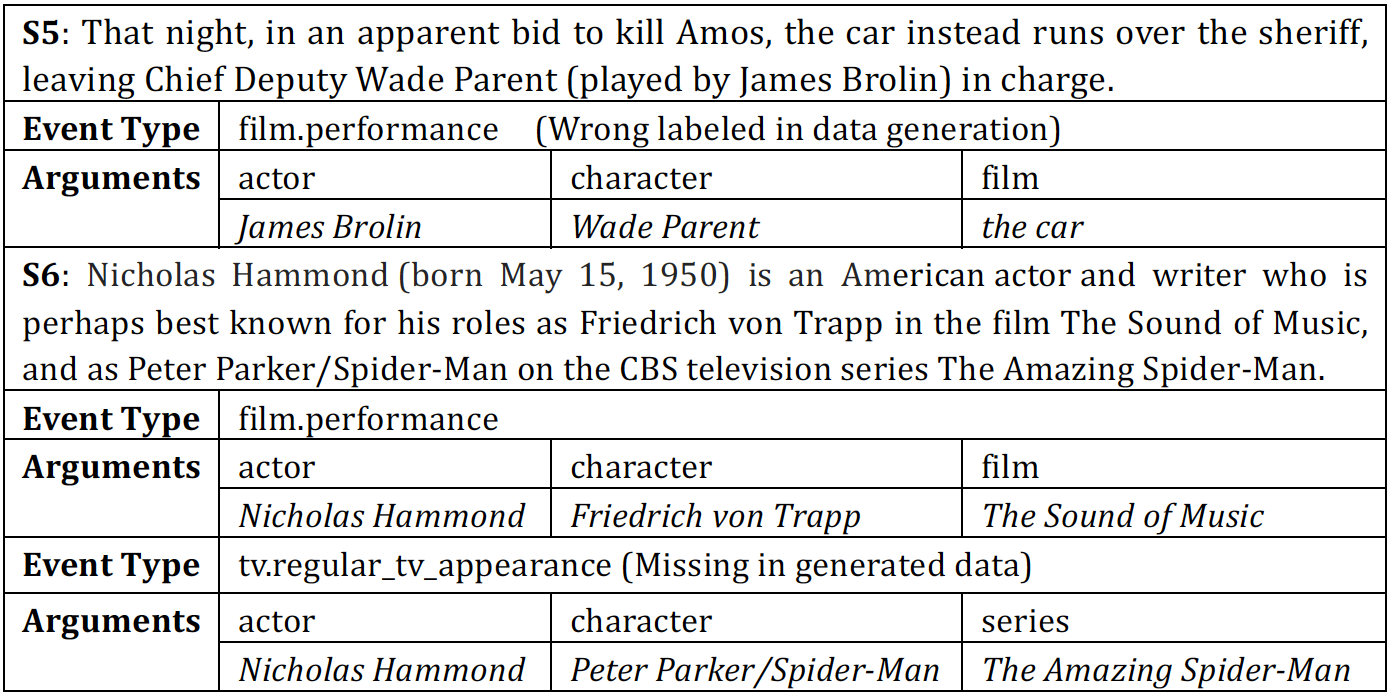
\includegraphics[width=.48\textwidth]{example.png}
	\caption{Example outputs of LSTM-CRF-ILP$_{multi}$.\label{fig:1}}
\end{figure}

Moreover, manual evaluation helps us to gain a deep insight of our data and models. We further conduct automatic evaluation on the manually annotated dataset and list the top 5 event types whose F1 scores of LSTM-CRF-ILP$_{multi}$ differ greatly from automatic evaluation in Table~\ref{tab:4}.

Most of the performance differences are caused by data generation. Figure~\ref{fig:1} examples two types of errors in data generation. Some automatically labeled sentences do not imply any event while still matching all key properties of certain instances. Take S5 as an example. Although the phrase \emph{the car} matches a film name, it does not indicate this film, and there is no explicit evidence expressing that an actor starring in a film. This is a bottleneck of our data generation strategy. During manual evaluation, we find 16 negative sentences which are mistakenly labeled due to this reason. Unfortunately, our model fails to rectify 10 of them.

Remarkably, our LSTM-CRF-ILP$_{multi}$ model can help find more CVT instances that are not referenced in Freebase. There are two events mentioned in S6, while the arguments of the second event do not match any CVT instances in Freebase, leading to a missing event in data generation. This phenomenon suggests that learning from distant supervision provided by Freebase, our model can help complete and update properties of Freebase instances in return.

\begin{table}[h]
\small
\centering
\begin{tabular}{|l|c|c|c|} \hline
	Event type & P & R & F \\ \hline
	olympics.medal\_honor%\footnote{The full name is olympics.olympic\_medal\_honor in Freebase.}
	& $\downarrow$ 25.0\% & $\downarrow$ 5.0\% & $\downarrow$ 13.8\% \\ \hline
	film.performance & $\downarrow$ 21.4\% & $\uparrow$ 3.1\% & $\downarrow$10.3\% \\ \hline
	business.acquisition & $\rightarrow$ & $\downarrow$ 7.1\% & $\downarrow$ 5.4\% \\ \hline
	tv.appearance%\footnote{The full name is tv.regular\_tv\_appearance in Freebase.}
	& $\downarrow$ 9.5\% & $\uparrow$ 3.0\% & $\downarrow$ 3.1\% \\ \hline
	film.release%\footnote{The full name is film.film\_regional\_release\_date in Freebase.}
	& $\downarrow$ 7.7\% & $\uparrow$ 5.6\% & $\downarrow$ 0.55\% \\ \hline
\end{tabular}
\caption{Top 5 event types whose performances on event classification differ most from automatic evaluation. The evaluated model is LSTM-CRF-ILP$_{multi}$ \label{tab:4}}
\end{table}

\subsection{Tables as Supervision}
To demonstrate the applicability of our approach to other structured tables besides Freebase CVT tables, we conduct manual evaluation on a new auto-annotated dataset with supervision provided by large Wikipedia tables. We acquire three tables characterizing events about acquisition, winning the Olympics, and winning the prestigious awards in entertainment industry. To evaluate the performance, we randomly select 100 sentences and follow the same steps of event annotations as mentioned in Section~\ref{manualeve}. 

\begin{table}[h]
\small
\centering
\begin{tabular}{|l|c|c|c|c|c|} \hline
	Event type & Table size & Dataset & EC & AD & ED \\ \hline
	Acquisition & 690 & 414 & 87.0 & 72.0 & 69.6 \\ \hline
	Olympics & 2503 & 1460 & 77.2 & 64.5 & 38.6 \\ \hline
	Awards & 3039 & 2217 & 95.0 & 82.8 & 58.6 \\ \hline
\end{tabular}
\caption{Statistics of the dataset and overall performance of our LSTM-CRF-ILP$_{multi}$ model. \textit{Table size} is the number of table entries. \textit{Dataset} is the size of training set. \label{tab:6}}
\end{table}

Table~\ref{tab:6} demonstrates that our approach with tabular data as distant supervision can be adapted to extract high-confidence events. Given a specific event type, as long as we acquire tables implying events of such type, we can construct a dataset and train an effective event extractor, which is much easier than human annotation and unlimited in event types. 
